\documentclass[tikz,border=3pt]{standalone}
\usetikzlibrary{patterns,shadings,decorations.pathmorphing}
\begin{document}
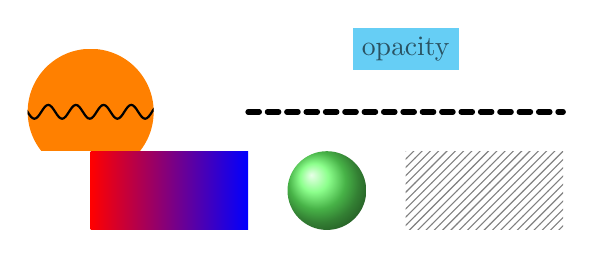
\begin{tikzpicture}
  \shade[left color=red,right color=blue] (0,0) rectangle (2,1);
  \shade[ball color=green!60] (3,0.5) circle (0.5);
  \fill[pattern=north east lines,pattern color=gray] (4,0) rectangle (6,1);
  \begin{scope}
    \clip (0,1.5) circle (0.8);
    \fill[orange] (-1,1) rectangle (1,2.3);
    \draw[decorate,decoration=snake,thick] (-1,1.5) -- (1,1.5);
  \end{scope}
  \draw[line width=2pt,line cap=round,dash pattern=on 4pt off 3pt] (2,1.5) -- (6,1.5);
  \node[opacity=0.6,fill=cyan,text=black] at (4,2.3) {opacity};
\end{tikzpicture}
\end{document}
